\DiaryEntry{Downsampling (revisited)}{2021-12-01}{Coding}

Let's consider the downsampling of a signal $x[n]$ in more detail. DOwnsampling means that we keep only every $m$-th sample in order to derive the signal $y[n]$,

\bee
y[n] = x[Mn]
\eee

This means that only samples of $x[n]$ are kept which occur at times equals to multiples of $M$ (with $M$ being an integer). This is shown in the following Figure (for $M = 2$).


\begin{figure}[H]
    \centering
    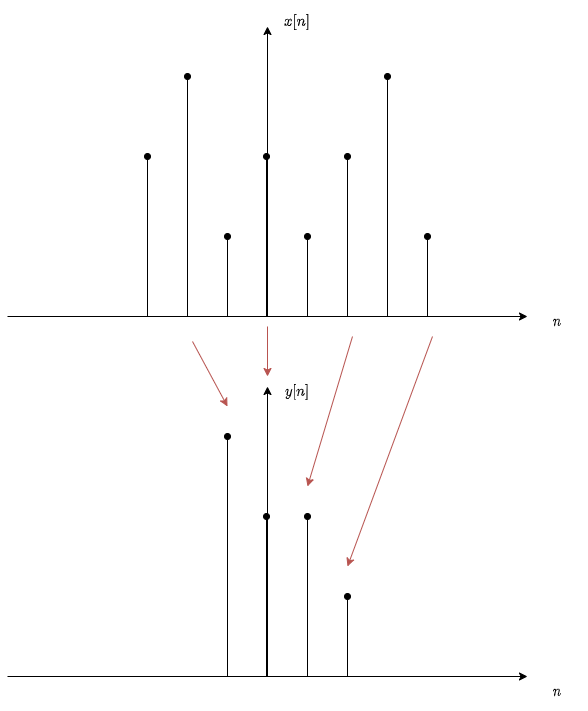
\includegraphics[scale=0.4]{images/2021-12-01-downsampling_1.png}
\end{figure}

We now calculate the z-transform of $y[n]$ (as function of $X(z)$),
\bee
Y(z) = \sum_n y[n] z^{-n} = \sum_n x[nM] z^{-n}
\eee

We next define an auxilary sequence

\bee
x_1[n] = \begin{cases} x[n] & n = kM \\
  0 & \text{otherwise} \end{cases}
\eee

and this allows us to further express $Y(z)$ as

\bee
Y(z) = \sum_n x[nM] z^{-n} = \sum_n x_1[n] z^{-n/M} = X_1(z^{1/M})
\eee

which is allowed because $x_1[n]$ is only non-zero at multiples of $M$. Now we tackle the z-transform of $x_1$. We write $x_1[n]$ as a product

\bee
x_1[n] = c[n] x[n]
\eee

where $c[n]$ is a pulse-train defined as

\bee
c[n] = \begin{cases} 1 & n = kM \\
  0 & \text{otherwise} \end{cases}
\eee

We can alternatively express this pulse-train as (see next Section) as

\bee
c[n] = \frac{1}{M} \sum_{k=0}^{M-1} W_M^{-kn}
\eee

and obtain

\bee
x_1[n] = x[n] \frac{1}{M} \sum_{k=0}^{M-1} W_M^{-kn} = \frac{1}{M} \sum_{k=0}^{M-1} x[n] W_M^{-kn}
\eee

The z-transform of $x_1[n]$ then becomes

\bee
X_1(z) = \sum_{n=-\infty}^\infty x_1[n] z^{-n} = \frac{1}{M} \sum_{n= -\infty}^\infty \sum_{k=0}^{M-1} x[n] W_M^{-kn} z^{-n} = \frac{1}{M} \sum_{k=0}^{M-1} \sum_{n= -\infty}^\infty x[n] (z W_M^k)^{-n} 
\eee

The inner sum can be read as z-transform

\bee
\sum_{n= -\infty}^\infty x[n] (zW^k)^{-n} = X(z W^k)
\eee

and therefore we have

\bee
Y(z) = \frac{1}{M} \sum_{k=0}^{M-1} X(z^{1/M} W^k) \qed
\eee

For the special case of $M = 2$, we have $W = -1$ and therefore

\bee
Y(z) = \frac{1}{2} X(z^{1/2}) + \frac{1}{2} X(-z^{1/2})
\eee



\subsection{Discrete-time Impulse Train}

We have an impulse train defined according to

\bee
c[n] = \sum_{k=-\infty}^\infty \delta[k-nM]
\eee

This is a periodic signal with period $M$. We can also express this signal by means of a \emph{discrete fourier series (DFS)}

\bee
c[n] = \frac{1}{M} \sum_{k=0}^{M-1} C[k] e^{j 2\pi/Nnk}
\eee

with fourier coefficients $C[k]$ given by

\bee
C[k] = \sum_{n=0}^{M-1} c[n] e^{- j 2\pi/Nnk}
\eee

For our impulse train, the fourier coefficients become

\bee
C[k] = e^{- j 2\pi/N 0 k} = 1 \quad \forall k
\eee

as the only non-zero contribution of $c[n]$ is at $n=0$. Therefore, we can express $c[n]$ as

\bee
c[n] = \frac{1}{M} \sum_{k=0}^{M-1} e^{j 2\pi/Nnk} = \frac{1}{M} \sum_{k=0}^{M-1} W_M^{-kn}
\eee

where $W_M$ defines the $M$-th root of unit given by $W_M = e^{-j 2\pi/M}$.



%%% Local Variables:
%%% mode: latex
%%% TeX-master: "journal"
%%% End:
